% Options for packages loaded elsewhere
\PassOptionsToPackage{unicode}{hyperref}
\PassOptionsToPackage{hyphens}{url}
\PassOptionsToPackage{dvipsnames,svgnames,x11names}{xcolor}
%
\documentclass[
  letterpaper,
  DIV=11,
  numbers=noendperiod]{scrartcl}

\usepackage{amsmath,amssymb}
\usepackage{lmodern}
\usepackage{iftex}
\ifPDFTeX
  \usepackage[T1]{fontenc}
  \usepackage[utf8]{inputenc}
  \usepackage{textcomp} % provide euro and other symbols
\else % if luatex or xetex
  \usepackage{unicode-math}
  \defaultfontfeatures{Scale=MatchLowercase}
  \defaultfontfeatures[\rmfamily]{Ligatures=TeX,Scale=1}
\fi
% Use upquote if available, for straight quotes in verbatim environments
\IfFileExists{upquote.sty}{\usepackage{upquote}}{}
\IfFileExists{microtype.sty}{% use microtype if available
  \usepackage[]{microtype}
  \UseMicrotypeSet[protrusion]{basicmath} % disable protrusion for tt fonts
}{}
\makeatletter
\@ifundefined{KOMAClassName}{% if non-KOMA class
  \IfFileExists{parskip.sty}{%
    \usepackage{parskip}
  }{% else
    \setlength{\parindent}{0pt}
    \setlength{\parskip}{6pt plus 2pt minus 1pt}}
}{% if KOMA class
  \KOMAoptions{parskip=half}}
\makeatother
\usepackage{xcolor}
\setlength{\emergencystretch}{3em} % prevent overfull lines
\setcounter{secnumdepth}{-\maxdimen} % remove section numbering
% Make \paragraph and \subparagraph free-standing
\ifx\paragraph\undefined\else
  \let\oldparagraph\paragraph
  \renewcommand{\paragraph}[1]{\oldparagraph{#1}\mbox{}}
\fi
\ifx\subparagraph\undefined\else
  \let\oldsubparagraph\subparagraph
  \renewcommand{\subparagraph}[1]{\oldsubparagraph{#1}\mbox{}}
\fi


\providecommand{\tightlist}{%
  \setlength{\itemsep}{0pt}\setlength{\parskip}{0pt}}\usepackage{longtable,booktabs,array}
\usepackage{calc} % for calculating minipage widths
% Correct order of tables after \paragraph or \subparagraph
\usepackage{etoolbox}
\makeatletter
\patchcmd\longtable{\par}{\if@noskipsec\mbox{}\fi\par}{}{}
\makeatother
% Allow footnotes in longtable head/foot
\IfFileExists{footnotehyper.sty}{\usepackage{footnotehyper}}{\usepackage{footnote}}
\makesavenoteenv{longtable}
\usepackage{graphicx}
\makeatletter
\def\maxwidth{\ifdim\Gin@nat@width>\linewidth\linewidth\else\Gin@nat@width\fi}
\def\maxheight{\ifdim\Gin@nat@height>\textheight\textheight\else\Gin@nat@height\fi}
\makeatother
% Scale images if necessary, so that they will not overflow the page
% margins by default, and it is still possible to overwrite the defaults
% using explicit options in \includegraphics[width, height, ...]{}
\setkeys{Gin}{width=\maxwidth,height=\maxheight,keepaspectratio}
% Set default figure placement to htbp
\makeatletter
\def\fps@figure{htbp}
\makeatother

<style>
.right {
  text-align: right;
}
</style>
\KOMAoption{captions}{tableheading}
\makeatletter
\makeatother
\makeatletter
\makeatother
\makeatletter
\@ifpackageloaded{caption}{}{\usepackage{caption}}
\AtBeginDocument{%
\ifdefined\contentsname
  \renewcommand*\contentsname{Table of contents}
\else
  \newcommand\contentsname{Table of contents}
\fi
\ifdefined\listfigurename
  \renewcommand*\listfigurename{List of Figures}
\else
  \newcommand\listfigurename{List of Figures}
\fi
\ifdefined\listtablename
  \renewcommand*\listtablename{List of Tables}
\else
  \newcommand\listtablename{List of Tables}
\fi
\ifdefined\figurename
  \renewcommand*\figurename{Figure}
\else
  \newcommand\figurename{Figure}
\fi
\ifdefined\tablename
  \renewcommand*\tablename{Table}
\else
  \newcommand\tablename{Table}
\fi
}
\@ifpackageloaded{float}{}{\usepackage{float}}
\floatstyle{ruled}
\@ifundefined{c@chapter}{\newfloat{codelisting}{h}{lop}}{\newfloat{codelisting}{h}{lop}[chapter]}
\floatname{codelisting}{Listing}
\newcommand*\listoflistings{\listof{codelisting}{List of Listings}}
\makeatother
\makeatletter
\@ifpackageloaded{caption}{}{\usepackage{caption}}
\@ifpackageloaded{subcaption}{}{\usepackage{subcaption}}
\makeatother
\makeatletter
\@ifpackageloaded{tcolorbox}{}{\usepackage[many]{tcolorbox}}
\makeatother
\makeatletter
\@ifundefined{shadecolor}{\definecolor{shadecolor}{rgb}{.97, .97, .97}}
\makeatother
\makeatletter
\makeatother
\ifLuaTeX
  \usepackage{selnolig}  % disable illegal ligatures
\fi
\IfFileExists{bookmark.sty}{\usepackage{bookmark}}{\usepackage{hyperref}}
\IfFileExists{xurl.sty}{\usepackage{xurl}}{} % add URL line breaks if available
\urlstyle{same} % disable monospaced font for URLs
\hypersetup{
  pdftitle={LAS 6292: Introduction},
  colorlinks=true,
  linkcolor={blue},
  filecolor={Maroon},
  citecolor={Blue},
  urlcolor={Blue},
  pdfcreator={LaTeX via pandoc}}

\title{LAS 6292: Introduction}
\author{}
\date{}

\begin{document}
\maketitle
\ifdefined\Shaded\renewenvironment{Shaded}{\begin{tcolorbox}[borderline west={3pt}{0pt}{shadecolor}, breakable, enhanced, interior hidden, sharp corners, boxrule=0pt, frame hidden]}{\end{tcolorbox}}\fi

\hypertarget{section}{%
\subsection{}\label{section}}

\hypertarget{introductions}{%
\subsubsection{INTRODUCTIONS}\label{introductions}}

\begin{itemize}
\tightlist
\item
  Name
\item
  In what city were you born?
\item
  What you consider your ``hometown''?
\item
  Program and Degree?
\item
  Hobbies or what you do to relax
\end{itemize}

\hypertarget{discuss}{%
\subsubsection{DISCUSS}\label{discuss}}

\begin{itemize}
\tightlist
\item
  Motivation for taking the class
\item
  Concerns about this class (in particular) and this semester (in
  general)?
\item
  Big Question on the next slide\^{}{[}Record all this to report back to
  the group{]}
\end{itemize}

\hypertarget{what-are}{%
\subsection{What are}\label{what-are}}

`DATA'?

\hypertarget{so-then}{%
\subsection{So then\ldots{}}\label{so-then}}

\hypertarget{what-are-1}{%
\subsection{What are}\label{what-are-1}}

`DATA'?

\hypertarget{section-1}{%
\subsection{}\label{section-1}}

\hypertarget{section-2}{%
\subsection{}\label{section-2}}

\hypertarget{section-3}{%
\subsection{}\label{section-3}}

\hypertarget{section-4}{%
\subsection{}\label{section-4}}

\hypertarget{section-5}{%
\subsection{}\label{section-5}}

``Anything you perform analysis on.''

\emph{Kristen Briney, p.~6}

\hypertarget{with-that-in-mind}{%
\subsection{With that in mind\ldots{}}\label{with-that-in-mind}}

\hypertarget{identify-different-kinds-of-data-collected-in-different-disciplines.}{%
\subsubsection{1. Identify different kinds of data collected in
different
disciplines.}\label{identify-different-kinds-of-data-collected-in-different-disciplines.}}

\hypertarget{how-are-these-data-collected-recorded}{%
\subsubsection{2. How are these data collected \&
recorded?}\label{how-are-these-data-collected-recorded}}

\emph{But first\ldots{}}

\begin{center}\rule{0.5\linewidth}{0.5pt}\end{center}

\hypertarget{section-6}{%
\subsection{}\label{section-6}}

What is

\emph{MY}

motivation?

\emph{\textbf{short answer:} data management might be the most important
skill you learn at UF}

\hypertarget{longer-answer-part-1}{%
\subsection{\texorpdfstring{\textbf{Longer answer:} Part
1}{Longer answer: Part 1}}\label{longer-answer-part-1}}

\hypertarget{section-7}{%
\subsection{}\label{section-7}}

\hypertarget{section-8}{%
\subsection{}\label{section-8}}

\hypertarget{section-9}{%
\subsection{}\label{section-9}}

\hypertarget{section-10}{%
\subsection{}\label{section-10}}

\hypertarget{section-11}{%
\subsection{---}\label{section-11}}

\hypertarget{section-12}{%
\subsection{---}\label{section-12}}

\hypertarget{section-13}{%
\subsection{---}\label{section-13}}

\hypertarget{longer-answer-part-3}{%
\subsection{\texorpdfstring{\textbf{Longer answer:} Part
3}{Longer answer: Part 3}}\label{longer-answer-part-3}}

---

\hypertarget{section-14}{%
\subsection{}\label{section-14}}

\hypertarget{section-15}{%
\subsection{}\label{section-15}}

\hypertarget{section-16}{%
\subsection{}\label{section-16}}

\hypertarget{longer-answer-part-3-1}{%
\subsection{\texorpdfstring{\textbf{Longer answer:} Part
3}{Longer answer: Part 3}}\label{longer-answer-part-3-1}}

\hypertarget{section-17}{%
\subsection{}\label{section-17}}

\hypertarget{section-18}{%
\subsection{}\label{section-18}}

\hypertarget{section-19}{%
\subsection{}\label{section-19}}

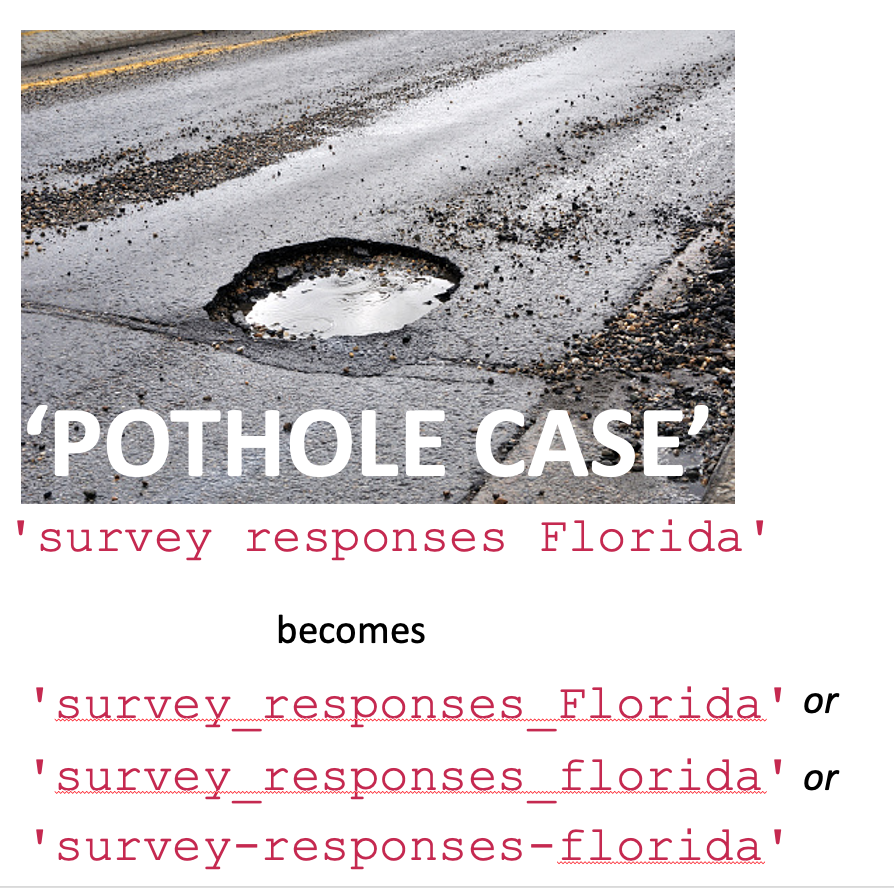
\includegraphics[width=0.7\textwidth,height=0.7\textheight]{./slide-images/img20.png}

Putz, F.E., Biotropica, 1983

\emph{(courtesy of FE Putz)}

\hypertarget{section-20}{%
\subsection{}\label{section-20}}

\emph{With that in mind\ldots{}}

\begin{enumerate}
\def\labelenumi{\arabic{enumi}.}
\tightlist
\item
  Identify different kinds of data collected in different disciplines.
\end{enumerate}

\begin{enumerate}
\def\labelenumi{\arabic{enumi}.}
\setcounter{enumi}{1}
\tightlist
\item
  How are these data collected \& recorded?
\end{enumerate}

\emph{(also\ldots time for a break!)}

\hypertarget{section-21}{%
\subsection{}\label{section-21}}

\hypertarget{section-22}{%
\subsection{}\label{section-22}}

\hypertarget{section-23}{%
\subsection{}\label{section-23}}

\begin{center}\rule{0.5\linewidth}{0.5pt}\end{center}

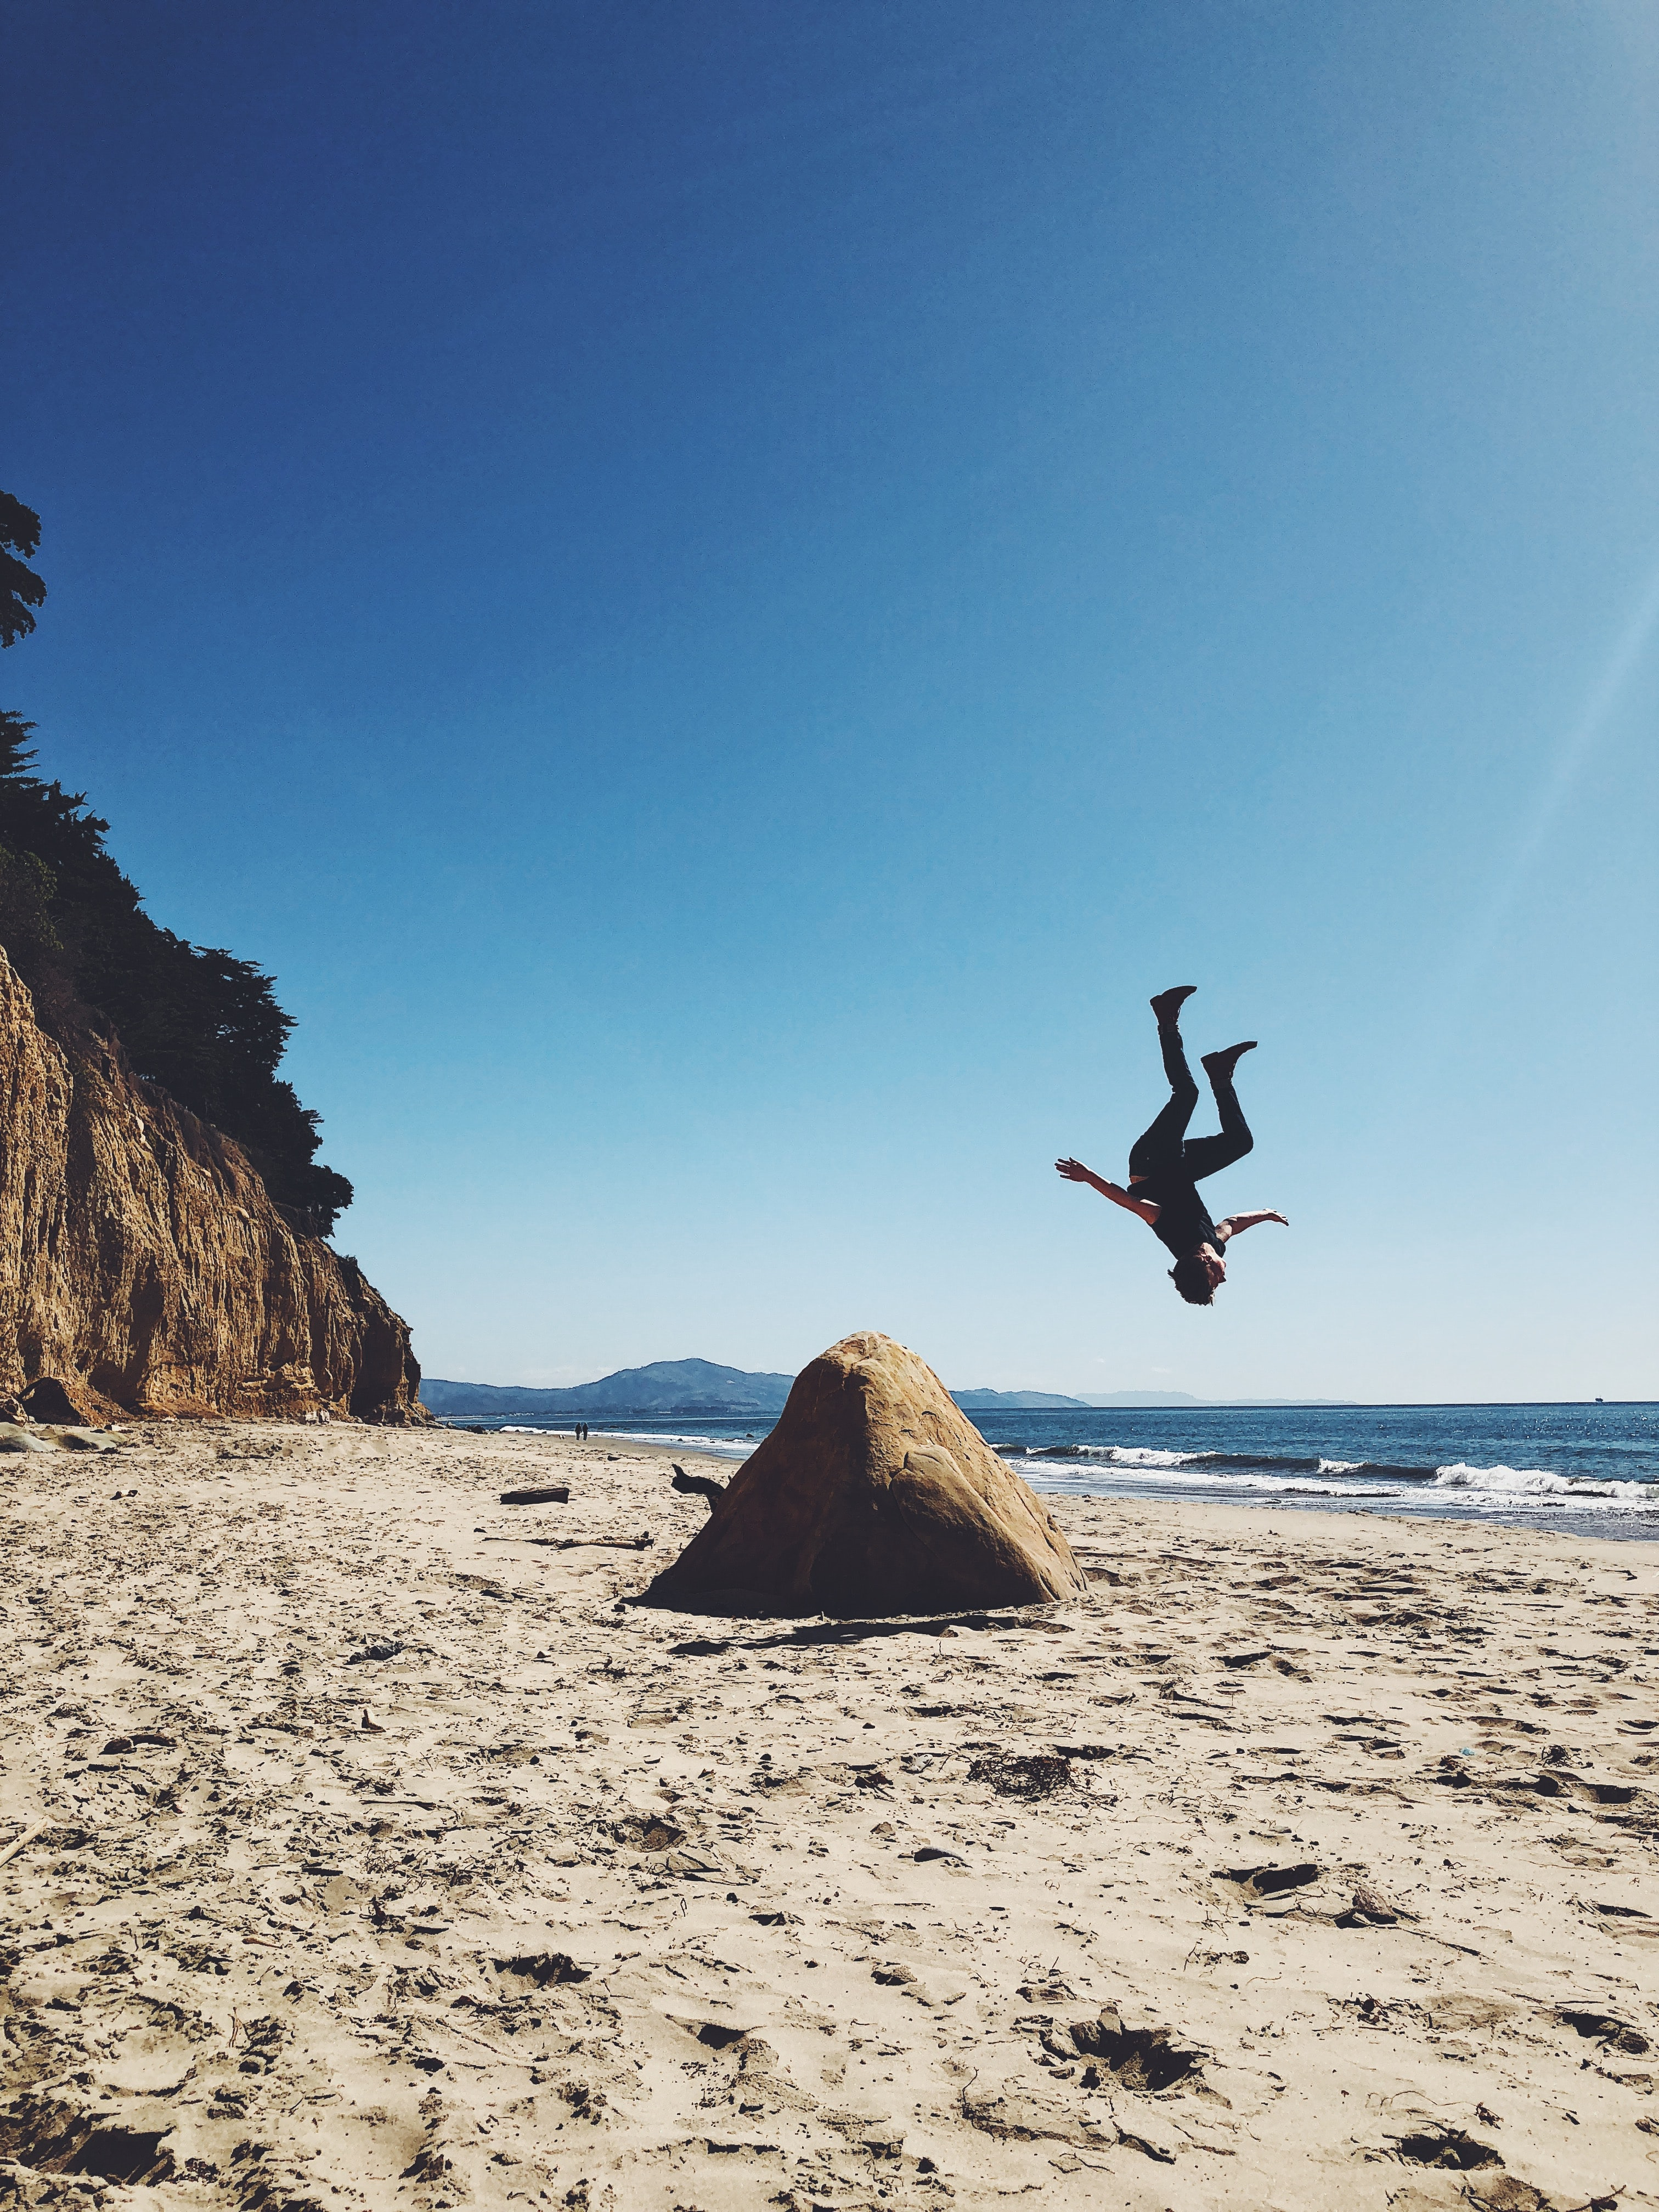
\includegraphics{./slide-images/chase-moyer-wRcwv-z6RDY-unsplash.png}

\textbf{Before Class}

\emph{Read, Watch, Reflect}

\textbf{During Class}

\emph{Exercises to Reinforce key ideas}

\emph{Discussion of Readings}

\emph{Work on Individual Project}

\begin{center}\rule{0.5\linewidth}{0.5pt}\end{center}

\hypertarget{lets-find-out-a-little-more}{%
\subsection{Let's find out a little
more\ldots{}}\label{lets-find-out-a-little-more}}

\hypertarget{in-class-exercise-wk.-1}{%
\subsubsection{\texorpdfstring{\emph{In-Class Exercise Wk.
1}}{In-Class Exercise Wk. 1}}\label{in-class-exercise-wk.-1}}

\emph{Work on Individual Project}



\end{document}
